% Section 3: Study Design
% Source: context/Empirical Evaluation Design (full)
% Source: context/Statistical Analysis Plan (full)
% Source: context/Paper_Layout_Plan.md §3
%
% EM-DASH PROHIBITION: Do not use --- or \textemdash. Use colons or semicolons.

\section{Study Design}\label{sec:study_design}

The goal is to establish that JWT relay corruption is systematic
(not model-specific), to quantify the limits of prompt-based mitigation, and to
validate an architectural solution in production. A controlled
experiment~\cite{shull2008guide} measures prevalence and effect sizes; an industrial case
study~\cite{runeson2009case} provides contextual validation. The ecological
validity arm bridges the two using production artifacts within the controlled
framework.

The study follows Verdecchia and Bogner~\cite{verdecchia2025notes} and
Kitchenham et al.~\cite{kitchenham2001guidelines}.
Sections~\ref{sec:objects}--\ref{sec:analysis_plan} describe the experiment;
Section~\ref{sec:case_study} presents the case study design and findings
together~\cite{runeson2009case}. Figure~\ref{fig:methodology} summarises the
overall process flow, from JWT generation through the main experiment and
ecological validity arms to statistical analysis; the industrial case study
(dashed, external) supplies the production tool schema that grounds the
ecological validity arm.

\begin{figure*}[t]
  \centering
  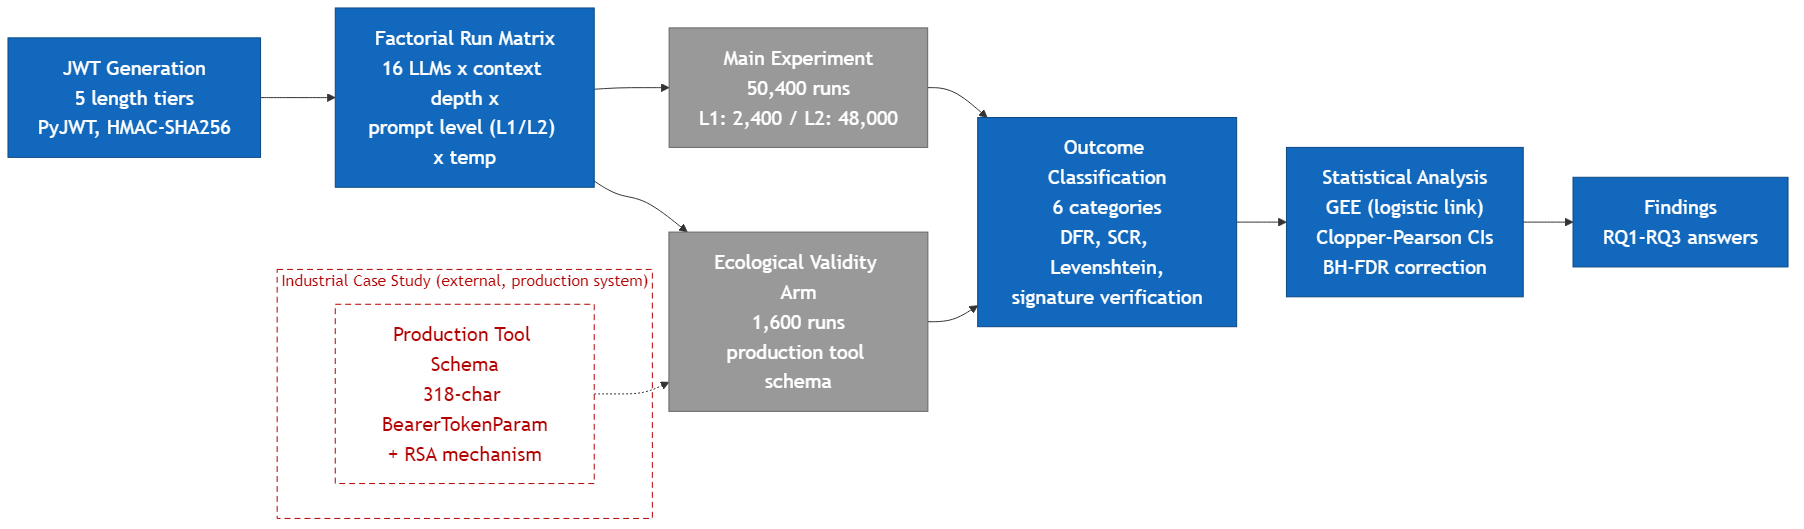
\includegraphics[width=0.75\textwidth]{figures/fig00_methodology_flow.png}
  \vspace{-4pt}\caption{Overall methodology process flow. Blue stages are
  common pipeline steps; grey stages are the two experimental arms. The
  dashed box denotes the industrial case study (Section~\ref{sec:case_study}),
  an external, production system that supplies the tool schema grounding the
  ecological validity arm.}
  \label{fig:methodology}
\end{figure*}

\subsection{Experimental Objects}\label{sec:objects}

The experimental objects are synthetic JWTs generated per-run using
\texttt{PyJWT} with a fresh HMAC-SHA256 secret and a randomised payload
containing a UUID, Unix timestamp, user identifier, and nested JSON claims.
Two design decisions motivate synthetic rather than real tokens. First, real
JWTs from known systems risk appearing in LLM training data, introducing a
contamination threat that synthetic tokens eliminate. Second, synthetic tokens
allow cryptographic signature verification as an independent ground-truth check
on corruption measurement.

JWTs are generated at five length tiers (Table~\ref{tab:jwt_tiers}) to test
the relationship between credential length and defect rate.

\begin{table}[t]
\centering
\small
\vspace{-4pt}\caption{JWT length tiers.}
\label{tab:jwt_tiers}
\begin{tabular}{@{}llp{3.8cm}@{}}
\toprule
\textbf{Tier} & \textbf{Target} & \textbf{Rationale} \\
\midrule
Short        & $\sim$200 chars & Minimal realistic JWT  \\
Medium low   & $\sim$300 chars & Below-typical; tests early-onset corruption \\
Medium       & $\sim$500 chars & Typical production JWT \\
Long         & $\sim$900 chars & Complex claims (e.g., role arrays) \\
Very long    & $\sim$1{,}400 chars & Upper extreme; production RS256 token ($\sim$1{,}080 chars) falls in this tier \\
\bottomrule
\end{tabular}
\end{table}

\subsection{Experimental Subjects}\label{sec:subjects}

Sixteen LLMs were selected across eight tiers (Table~\ref{tab:models}) to
provide broad coverage of the 2026 frontier landscape. The selection follows
current guidelines for empirical SE studies involving
LLMs~\cite{verdecchia2025notes}, requiring commercial frontier models,
open-source baselines, and longitudinal pairs (two Claude Sonnet generations,
two Google Gemini generations) to test whether model-generation advancement
reduces corruption. Chinese and European frontier models are included because
different training corpora may produce tokenisers with different Base64url
segmentation behaviour.

\begin{table*}[t]
\centering
\small
\vspace{-4pt}\caption{Model taxonomy. All models were API-version pinned at the start of
data collection. Tier codes: WF=Western Frontier, CE=Cost-Efficient,
R=Reasoning, CF=Chinese Frontier, EF=European Frontier, LB=Legacy Baseline,
SL=Sonnet Longitudinal, GL=Google Longitudinal, LO=Local/Open-weight.}
\label{tab:models}
\setlength{\tabcolsep}{6pt}
\begin{tabular}{@{}lll@{\qquad\qquad}lll@{}}
\toprule
\textbf{Model} & \textbf{Tier} & \textbf{Provider} &
\textbf{Model} & \textbf{Tier} & \textbf{Provider} \\
\midrule
Claude Sonnet 5       & WF & Anthropic  & Mistral Large 3       & EF & Mistral \\
Gemini 3.5 Flash      & WF & Google     & Mistral Small 4       & EF & Mistral \\
GPT-5.4-mini          & CE & OpenAI     & GPT-4o (pinned)       & LB & OpenAI \\
Claude Haiku 4.5      & CE & Anthropic  & Claude Sonnet 4.5     & SL & Anthropic \\
Gemini 3.1 Flash-Lite & CE & Google     & Claude Sonnet 4.6     & SL & Anthropic \\
o4-mini               & R  & OpenAI     & Gemini 3 Flash        & GL & Google \\
DeepSeek V3           & CF & DeepSeek   & Gemini 2.5 Flash      & GL & Google \\
GLM-4 Flash           & CF & Zhipu AI   & Gemma 4 E4B           & LO & Ollama \\
\bottomrule
\end{tabular}
\end{table*}

\subsection{Variables}\label{sec:variables}

\textbf{Independent variables.}
The experiment uses a mixed factorial design:
(1)~JWT length tier (5~levels: short, medium-low, medium, long, very-long);
(2)~context depth (3~levels: shallow~$\sim$100 tokens, medium~$\sim$1{,}500,
    deep~$\sim$3{,}000 tokens);
(3)~prompt ecological level (2~levels: L1, L2);
and (4)~temperature ($T\!=\!0.0$ and $T\!=\!0.7$).
L2 was run at all factor combinations (100 iterations per cell); L1
at a single temperature and medium context depth to bound cost.
The 15 API-hosted models each completed 3{,}000 L2 target runs; Gemma~4~E4B
(Ollama local) completed 3{,}000 L2 runs, yielding 48{,}000 total L2 runs
(100\% of the 48{,}000 API-model target).
L1 contributed 2{,}400 runs (16 models $\times$ 150 iterations across five
JWT-length tiers, single temperature, medium context depth), bringing the
combined main-arm total to 50{,}400. With the eco arm ($N\!=\!1{,}600$;
Section~\ref{sec:eco_arm}), the overall study comprises 52{,}000 completed
runs.

\textbf{Dependent variables.}
The primary outcome is the \emph{Defect/Failure Rate} (\DFR{}): a binary
indicator coded 1 if the output does not byte-for-byte match the input JWT. For
corrupted runs, we compute the Levenshtein distance to measure severity and the
Segment Corruption Rate (SCR) per JWT segment (header, payload, signature).
Cryptographic signature verification provides an independent ground-truth check.

Outcomes are classified into six mutually exclusive categories
(Table~\ref{tab:taxonomy}, Section~\ref{sec:rq2}). \textit{Semantic
substitution} is assigned when the output contains no dot-separated
Base64url triplet but is non-empty (UUID extraction, JSON expansion,
claim-value repetition). The replication package contains verbatim
prompt templates, API model identifiers, SDK versions, tool schemas, request/response extraction, and error-handling
logic.

\subsection{Ecological Validity Arm}\label{sec:eco_arm}

To test whether prompt-engineering mitigations can close the gap under
production conditions, we conduct an ecological validity arm ($N\!=\!1{,}600$;
16 models $\times$ 100 iterations) using the exact JWT schema and the
verbatim 318-character \texttt{BearerTokenParam} tool instruction from the
production codebase (Section~\ref{sec:case_study}), which names the RSA
mechanism and warns that any single changed character produces a 403~error.
A \texttt{RESEARCH\_RAW\_MODE} flag bypasses production mitigations.
The pre-specified test is Spearman's $\rho$ between eco arm and main
experiment model rankings.

\subsection{Analysis Plan}\label{sec:analysis_plan}

Between-model inference uses Generalised Estimating Equations (GEE) with
logistic link, binomial family, and exchangeable working correlation, clustered
at the (model, cell) level. GEE estimates population-average effects and is
robust to correlation misspecification via the sandwich variance
estimator~\cite{kitchenham2001guidelines}. Per-model \DFR{} estimates use
Clopper-Pearson exact binomial 95\% confidence intervals. Pairwise comparisons
use Benjamini-Hochberg FDR correction at $\alpha\!=\!0.05$. The eco arm uses
Spearman's $\rho$ for rank correlation and Mann-Whitney~$U$ for the vocabulary
effect test.
